%----------------------------------------------------------------------------------------
%	PACKAGES AND THEMES
%----------------------------------------------------------------------------------------
\PassOptionsToPackage{table}{xcolor}
\documentclass[aspectratio=169,xcolor=dvipsnames,svgnames,x11names,fleqn]{beamer}
% \documentclass[aspectratio=169,xcolor=dvipsnames,fleqn]{beamer}

\usetheme{RedVelvet}

\usefonttheme[onlymath]{serif}
\newcommand{\showanswers}{yes}


\usepackage{xspace}
\usepackage{amsmath}
\usepackage{amssymb}
\usepackage{amsfonts}
\usepackage{color}
\usepackage{physics}
% \usepackage{mathbb}
\usepackage{rahul_math}
\usepackage{bigints}

\usepackage{graphicx} % Allows including images
\usepackage{booktabs} % Allows the use of \toprule, \midrule and \bottomrule in tables
\usepackage{tikz,pgfplots}

\usepackage{subfigure}
\usetikzlibrary{arrows}
\usepackage{minted}
\definecolor{LightGray}{gray}{0.9}
\definecolor{cream}{rgb}{0.92, 0.9, 0.55}
\definecolor{lightblue}{rgb}{0.68, 0.85, 0.9}


\usepackage{xcolor-material}
\usetikzlibrary{fit}
\usetikzlibrary{matrix}
\tikzset{%
apple/.pic={
    \fill [MaterialBrown] (-1/8,0)  arc (180:120:1 and 3/2) coordinate [pos=3/5] (@)-- ++(1/6,-1/7)  arc (120:180:5/4 and 3/2) -- cycle;
    \fill [MaterialLightGreen500] (0,-9/10)  .. controls ++(180:1/8) and ++(  0:1/4) .. (-1/3,  -1) .. controls ++(180:1/3) and ++(270:1/2) .. (  -1,   0) .. controls ++( 90:1/3) and ++(180:1/3) .. (-1/2, 3/4) .. controls ++(  0:1/8) and ++(135:1/8) .. (   0, 4/7)
    }
    }

\newcommand{\leftdoublequote}{\textcolor{blue}{\scalebox{3}{``}}}

\newcommand{\rightdoublequote}{\textcolor{blue}{\scalebox{3}{''}}}


\usepackage{textcomp}
\usepackage{fontawesome}
\usepackage{tikz,pgfplots}
\usetikzlibrary{shapes.callouts}
\usetikzlibrary{arrows}


\usepackage{overpic}

%----------------------------------------------------------------------------------------
%	TITLE PAGE
%----------------------------------------------------------------------------------------

\usepackage{tikz-qtree,tikz-qtree-compat}
\usetikzlibrary{tikzmark}
\usetikzlibrary{calc}


\title[CPE 486/586: Machine Learning]{CPE 486/586: Machine Learning for Engineers} % The short title appears at the bottom of every slide, the full title is only on the title page
\subtitle{10 Dimensionality Reduction}

\author[Rahul Bhadani] {{\Large \textbf{Rahul Bhadani}}}

\institute[UAH] % Your institution as it will appear on the bottom of every slide, maybe shorthand to save space
{
    Electrical \& Computer Engineering,  The University of Alabama in Huntsville
}
\date

% \titlegraphic{
%    \includegraphics[width=0.4\linewidth]{figures/UAH_primary.png}
% }

\begin{document}

%-------------------------------------------------
\begin{frame}
    \titlepage
\end{frame}

%-------------------------------------------------
\begin{frame}{Outline}
    \backgroundtableofcontents
\end{frame}



%%%%%%%%%%%%%%%%%%%%%%%%%%%%%%%%%%%%%%%%%%%%%%%%%%%%%
\begin{sectionframe}{\faFire}{Motivation}
\end{sectionframe}


\begin{frame}{Examples of High-Dimensional Data}
    \begin{itemize}
        \item High resolution images
    \end{itemize}

    
    
    \begin{columns}
        \column{0.1\linewidth}
        \column{0.4\linewidth}
        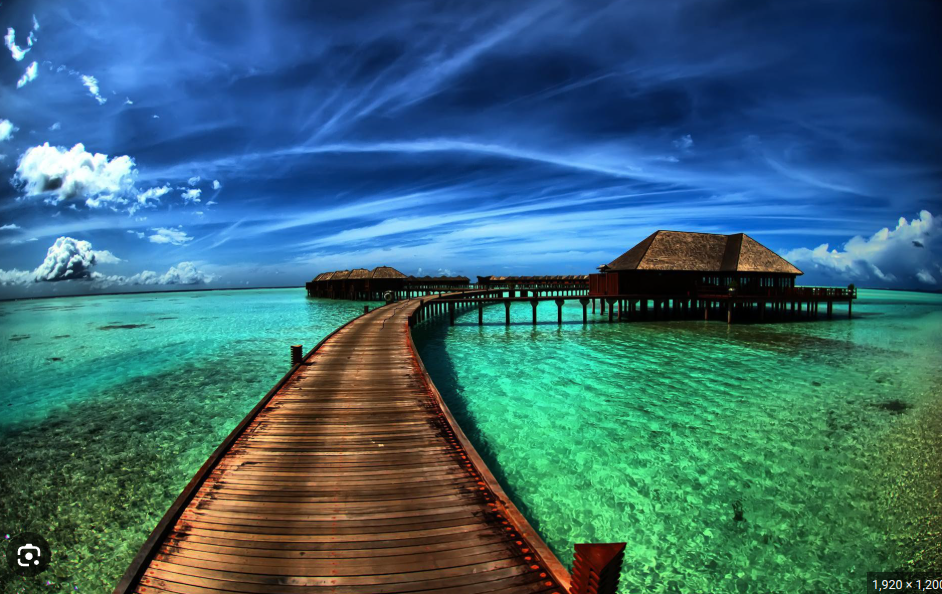
\includegraphics[width=0.99\textwidth]{figures/high-res1.png}

        \column{0.4\linewidth}
        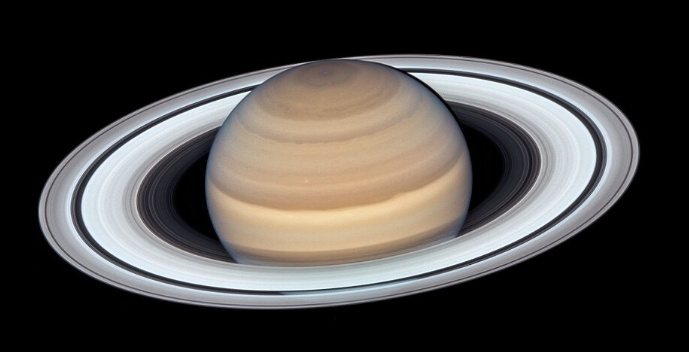
\includegraphics[width=0.99\textwidth]{figures/high-res2.png}
        \column{0.1\linewidth}

    \end{columns}

\end{frame}

\begin{frame}{Examples of High-Dimensional Data (cont.)}

    \begin{itemize}
        \item Customer Purchase Data

        
\includegraphics[width=0.59\textwidth, height=0.68\textheight, keepaspectratio]{figures/amazon.png}

    \end{itemize}
\end{frame}



\begin{frame}{Motivating Dimensionality Reduction}
\Large
\begin{itemize} 
    \item There is a {\color{MediumBlue}curse of dimensionality}! The complexity of a model increases with the dimensionality. Sometimes exponentially!
    \item So, why should we perform dimensionality reduction?
      \begin{itemize}\large
        \item reduces the time complexity: less computation
        \item reduces the space complexity: fewer parameters
        \item saves costs: some features/variables cost money 
         \item makes complex high-dimensional data easier to interpret
        \item Can you visualize data with more than three dimensions?
      \end{itemize}
\end{itemize}
\end{frame}


\begin{frame}{The Curse of Dimensionality in Numbers}
    \large
    Spread points uniformly in the unit hypercube $[0,1]^D$. A neighborhood that has 10\% of the data is a sub-cube with edge length
    \begin{multiequation}
        e_D = 0.1^{1/D}
    \end{multiequation}
    \begin{center}
    \renewcommand{\arraystretch}{1.3}
    \begin{tabular}{c|ccccc}
        $D$   & 1     & 2     & 3     & 10    & 100   \\ \hline
        $e_D$ & 0.100 & 0.316 & 0.464 & 0.794 & 0.977
    \end{tabular}
    \end{center}
    \begin{tblock}{Consequence}
        At $D = 10$ the ``local'' neighborhood covers 79\% of the range of a feature. At $D = 100$ it covers 98\%. A $k$-NN classifier then averages over points that lie far from the query.
    \end{tblock}
\end{frame}

\begin{frame}{Learning Representations}

    \begin{tblock}{Dimensionality Reduction Algorithms}

        Powerful, often unsupervised, learning techniques for extracting hidden
and potentially lower dimensional structure from high dimensional datasets.
        
    \end{tblock}

    Examples: 

       PCA, Kernel PCA, ICA, CCA, t-SNE, UMAP, Autoencoders, Matrix Factorization


    \textbf{Some advantage:}

    \begin{itemize}
        \item Better Visualization
        \item Efficient use of resources such as time, memory, communication
                \item Statistical: fewer parameters to fit, which reduces overfitting when the discarded directions carry noise
        \item Noise removal (improving data quality)
    \end{itemize}
    
\end{frame}

%%%%%%%%%%%%%%%%%%%%%%%%%%%%%%%%%%%%%%%%%%%%%%%%%%%%%
\begin{sectionframe}{\faCodepen}{Principal Component Analysis (PCA)}
\end{sectionframe}


\begin{frame}{PCA: Proposed more than 100 years ago!}
    
    \begin{columns}
        \column{0.1\linewidth}
        \column{0.4\linewidth}
        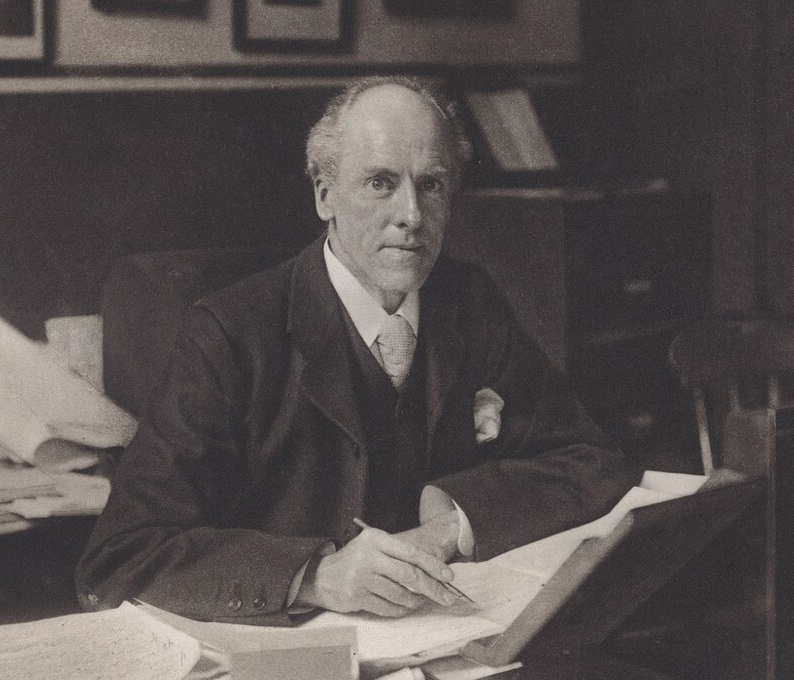
\includegraphics[width=0.69\textwidth]{figures/karl_pearson.jpg}

        Karl Pearson (invented in 1901)

        \column{0.4\linewidth}
        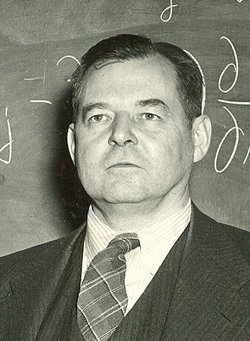
\includegraphics[width=0.5\textwidth]{figures/Harol_Hotelling.jpg}

        Harold Hotelling (named it principal components, 1933)

        \column{0.1\linewidth}

    \end{columns}

\end{frame}

\begin{frame}{Why?}

    \Large 

    \begin{itemize}
        \item Helpful for reducing number of features
        \item For 2D/3D visualization
        \item Helpful in unsupervised algorithms
        \item Data storage cost can be lowered
    \end{itemize}
    
\end{frame}

%------------------------------------------------

\begin{frame}{Intuition Behind PCA}
    \begin{columns}

    \column{0.6\textwidth}
    $x_1$: length of the car, $x_2$: width of the car

    {\color{lightgray}Class Work}



        \column{0.4\textwidth}
  \hfill  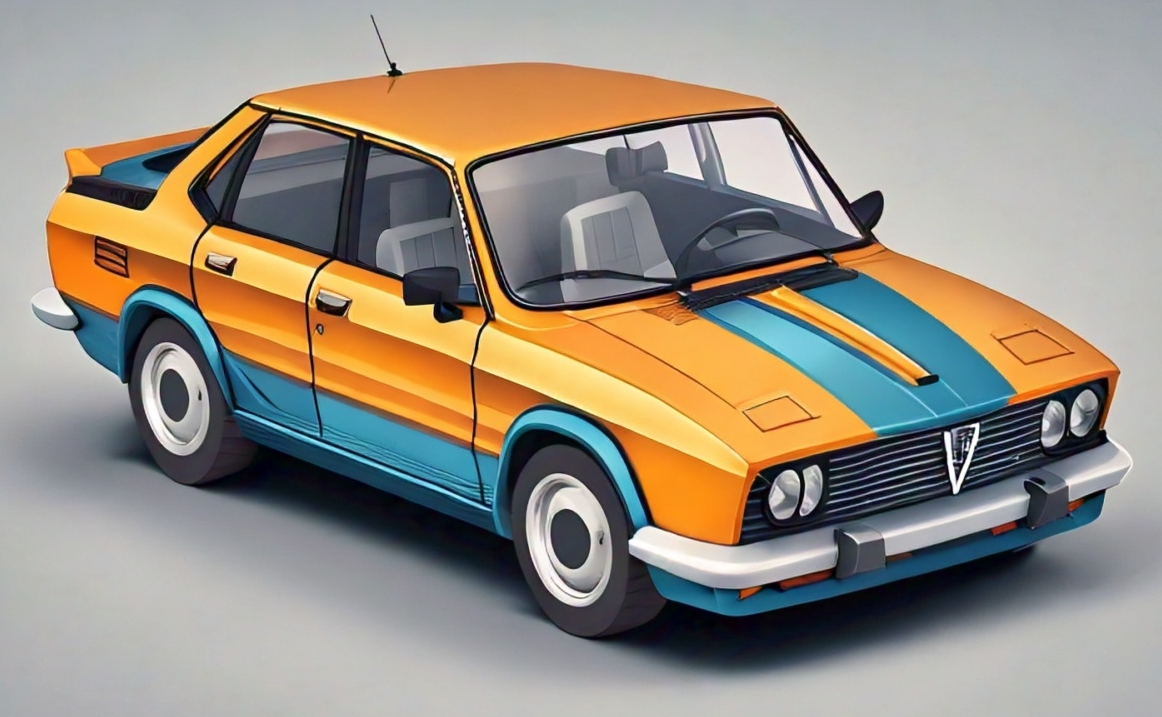
\includegraphics[width=0.99\textwidth]{figures/a_car.jpg}

    \end{columns}
\end{frame}

%------------------------------------------------

\begin{frame}{Intuition Behind PCA}
    \begin{columns}

    \column{0.6\textwidth}

    $x_1$: length of the car, $x_3$: diameter of the wheel

    {\color{lightgray}Class Work}
        \column{0.4\textwidth}
  \hfill  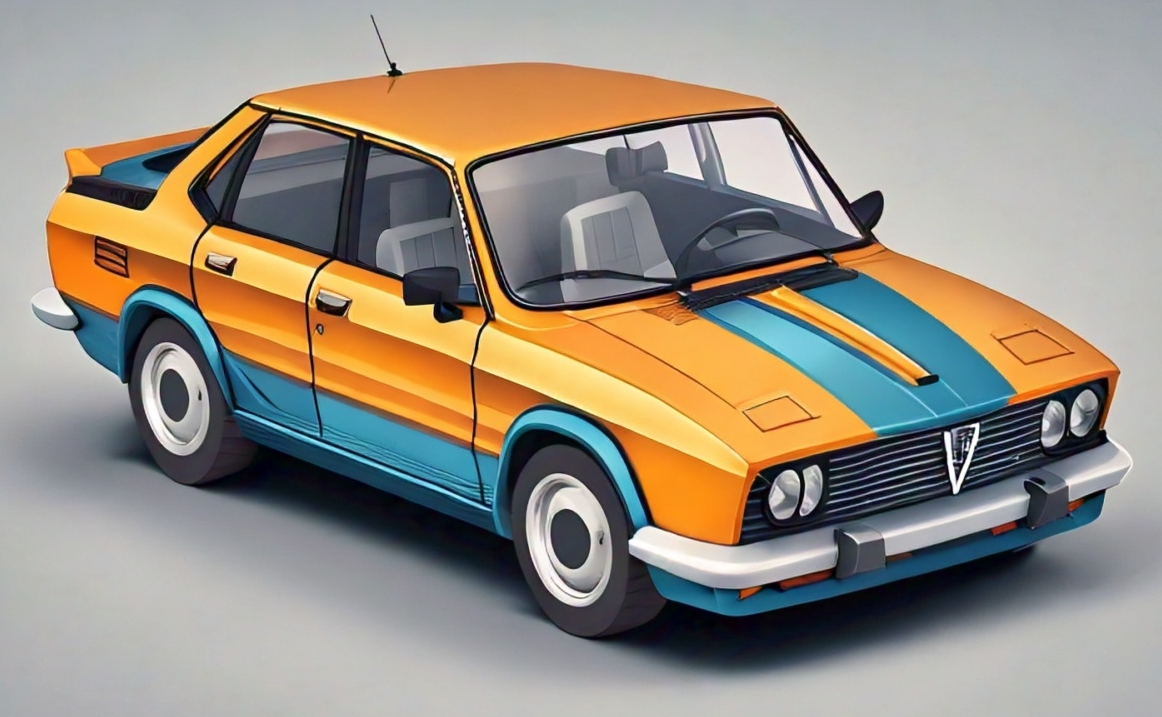
\includegraphics[width=0.99\textwidth]{figures/a_car.jpg}

    \end{columns}
\end{frame}

%------------------------------------------------

\begin{frame}{Intuition Behind PCA}
    \begin{columns}

    \column{0.6\textwidth}
    $x_1$: length of the car, $x_4$: height of the car


    {\color{lightgray}Class Work}
        \column{0.4\textwidth}
  \hfill  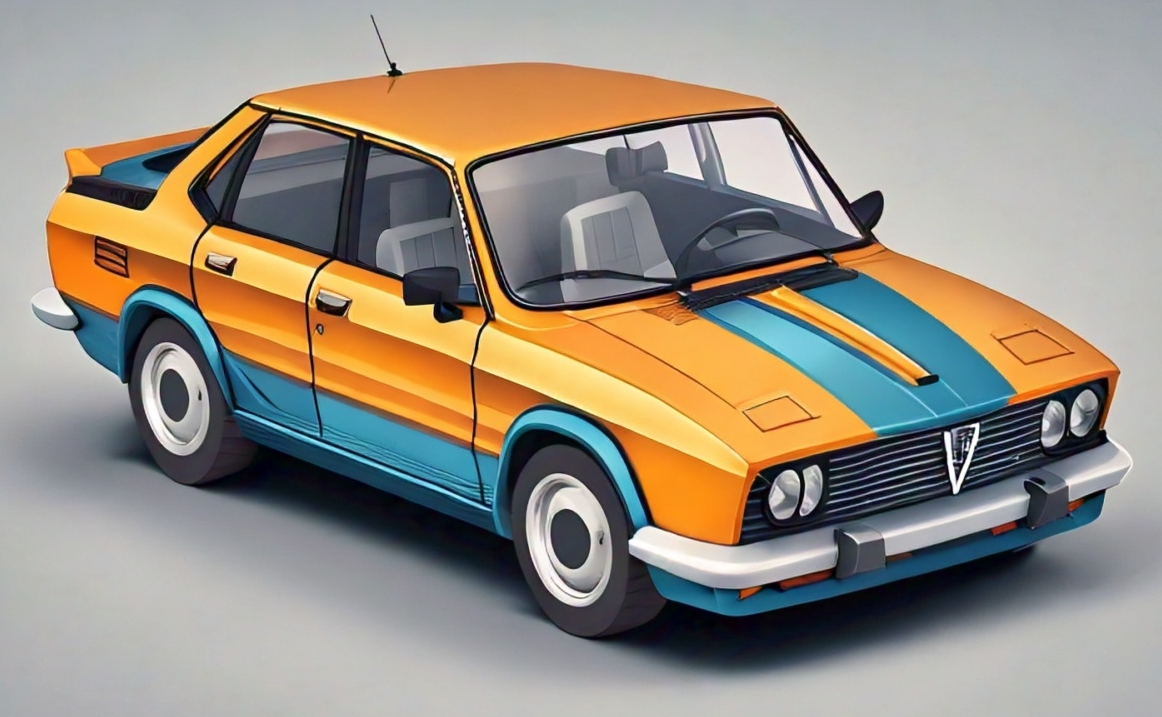
\includegraphics[width=0.99\textwidth]{figures/a_car.jpg}

    \end{columns}
\end{frame}

%------------------------------------------------

\begin{frame}{Problem Setting}

    \Large 
    \begin{center}
                We are interested in finding projections $\hat{\xbf}_i$ of data points $\xbf_i$ that are as similar to the original data points as possible, but which have significantly lower intrinsic dimensionality.
    \end{center}
    
    \begin{tblock}{Question}
            Given a dataset $X = \{ \xbf_1, \ldots, \xbf_N\}$, $\xbf_i\in \Rbb^D$, is there an $M$-dimensional subspace of $\Rbb^D$, $M \ll D$, in which $X$ approximately lies?
    \end{tblock}

\end{frame}


%------------------------------------------------

\begin{frame}{How does PCA work}
    \begin{columns}

    \column{0.6\textwidth}
    {\color{lightgray}Class Work}
        \column{0.4\textwidth}

    \end{columns}
\end{frame}

%------------------------------------------------

\begin{frame}{How does PCA work}
    \begin{columns}

    \column{0.6\textwidth}
    {\color{lightgray}Class Work}
        \column{0.4\textwidth}

    \end{columns}
\end{frame}

%------------------------------------------------

\begin{frame}{How does PCA work}
    \begin{columns}

    \column{0.6\textwidth}
    {\color{lightgray}Class Work}
     \column{0.4\textwidth}
       

    \end{columns}
\end{frame}


%%%%%%%%%%%%%%%%%%%%%%%%%%%%%%%%%%%%%%%%%%%%%%%%%%%%%
\begin{sectionframe}{\faPercent}{Mathematics behind PCA}
\end{sectionframe}

\begin{frame}{Feature Preprocessing}
   \begin{tblock}{}
       \begin{itemize}
                        \item Center the data so that the features have mean $0$.
           \begin{multiequation}
               \boldsymbol{\mu} & = \cfrac{1}{N}\sum_{i = 1}^N \xbf_i, \qquad \xbf_i \leftarrow \xbf_i-\boldsymbol{\mu}
            \end{multiequation}
            \item When the features carry different units, also scale them to $\sigma_j = 1$.
           \begin{multiequation}
               \sigma_j^2 & = \cfrac{1}{N}\sum_{i=1}^N x_{ij}^2, \qquad x_{ij} \leftarrow \cfrac{x_{ij}}{\sigma_j}
            \end{multiequation}
       \end{itemize}
   \end{tblock}
   After standardization, a speed recorded in km/h and again in mph gives two identical columns, and PCA merges them into one component.
\end{frame}

\begin{frame}{Covariance Matrix}

    \large

    We assume the samples $X = \{ \xbf_1, \ldots, \xbf_N \}$ are iid. After centering, they have mean $\mathbf{0}$ and covariance matrix
    \begin{multiequation}
        \Sigma = \cfrac{1}{N} \sum_{i=1}^N \xbf_i \xbf_i^\top \in \Rbb^{D\times D}
    \end{multiequation}

    Here $\xbf_i \in \Rbb^D$.
    
\end{frame}

\begin{frame}{Projecting onto New Axes}

    \begin{columns}
        \column{0.5\linewidth}
        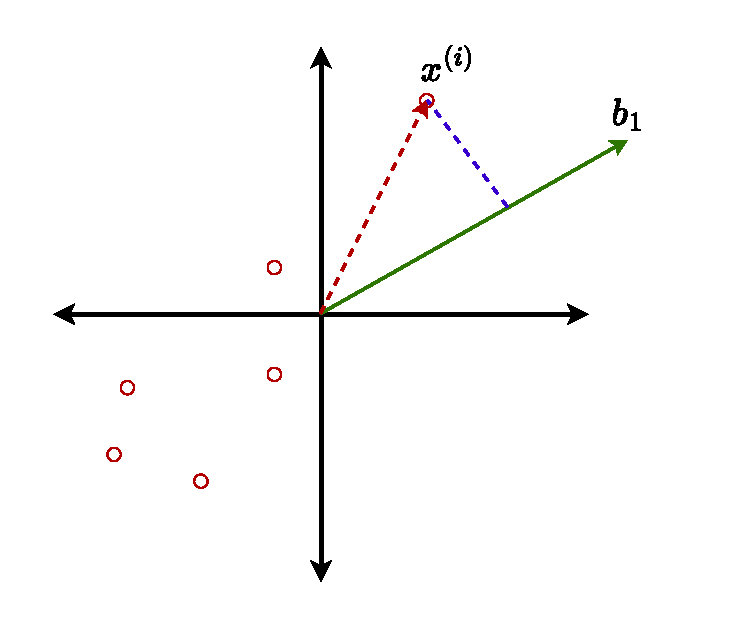
\includegraphics[width=0.99\textwidth]{figures/Projection.pdf}
        \column{0.5\linewidth}
        
        \large 

        The coordinates (the code) of $\xbf_i$ along the new axes $\bbf_1, \ldots, \bbf_M$ are
        $$
        \zbf_i = \Bbf^\top \xbf_i \in \Rbb^M
        $$
        with $\Bbf := [\bbf_1, \ldots, \bbf_M] \in \Rbb^{D\times M}$. The projection of $\xbf_i$ in $\Rbb^D$ is $\Bbf\Bbf^\top\xbf_i$.

        We assume that the columns of $\Bbf$ are orthonormal: $\|\bbf_k\| = 1$ and $\bbf_k^\top \bbf_l = 0$ for $k \neq l$.
    \end{columns}


\end{frame}



\begin{frame}{Find the Direction of Maximal Variance}
We maximize the variance of the low-dimensional code using a sequential approach. Start with a single vector $\bbf_1 \in \Rbb^D$ that maximizes the variance of the projected data.

\Large 
How do we choose unit vector $\bbf_1$ so that we maximize
$$
V = \cfrac{1}{N}\sum_{i=1}^N (\bbf_1^\top \xbf_i)^2
$$

The data are centered, so the projections $\bbf_1^\top\xbf_i$ have mean $0$ and their mean square is their variance.


\end{frame}

\begin{frame}{The Direction with Maximal Variance}

    \Large 
Expanding

\begin{multiequation}
V & = \cfrac{1}{N}\sum_{i=1}^N (\bbf_1^\top \xbf_i)^2 = \cfrac{1}{N}\sum_{i=1}^N \bbf_1^\top \xbf_i \xbf_i^\top \bbf_1 \\
    & = \bbf_1 ^\top \bigg( \cfrac{1}{N} \sum_{i=1}^N \xbf_i {\xbf_i}^\top \bigg)  \bbf_1 =  \bbf_1 ^\top \Sigma  \bbf_1 
\end{multiequation}

The dot product is symmetric, i.e. $ \bbf_1^\top \xbf_i = \xbf_i^\top \bbf_1 $.
\end{frame}

\begin{frame}{Lagrange Multiplier to Solve the Optimization Problem}
    
    \Large 
    Our goal is to maximize $ \bbf_1 ^\top \Sigma  \bbf_1 $
    such that
    $$
    \bbf_1^\top \bbf_1 = 1 \Rightarrow  \bbf_1^\top  \bbf_1 - 1 = 0
    $$
    We use the method of Lagrange Multiplier 
    $$
    \Lcal( \bbf_1, \lambda) =  \bbf_1^\top \Sigma  \bbf_1 - \lambda ( \bbf_1^\top  \bbf_1 - 1)
    $$
\end{frame}

\begin{frame}{Lagrange Multiplier to Solve the Optimization Problem}
\Large
\begin{columns}
    \column{0.60\linewidth}
    \begin{multiequation}
        \Lcal( \bbf_1, \lambda) & =  \bbf_1^\top \Sigma  \bbf_1 - \lambda ( \bbf_1^\top  \bbf_1 - 1)
    \end{multiequation}
    Take the gradient with respect to $ \bbf_1$

    \begin{multiequation}
        \nabla_{ \bbf_1}  \Lcal( \bbf_1, \lambda) & = 2\Sigma  \bbf_1 - 2\lambda  \bbf_1 = \mathbf{0}\\
        & \Rightarrow  \Sigma  \bbf_1 = \lambda \bbf_1
    \end{multiequation}

    \column{0.05\linewidth}
    \column{0.30\linewidth}
    We see that $\bbf_1$ is an eigenvector of the covariance matrix $\Sigma$ and the Lagrange multiplier $\lambda$ is the corresponding eigenvalue.

\end{columns}


\end{frame}

\begin{frame}{Eigenvalue Problem}

  
    From the eigenvector property:

    \begin{multiequation}
        V =  \bbf_1^\top \Sigma  \bbf_1 = \lambda  \bbf_1^\top  \bbf_1 = \lambda
    \end{multiequation}

    \begin{tblock}{}
    Hence, the variance of the data projected onto a 1-D subspace equals the eigenvalue associated with the basis vector $\bbf_1$ that spans the subspace.
    \end{tblock}

        To maximize the variance of the low-dimensional code, we choose the eigenvector associated with the largest eigenvalue $\lambda_1$ of the covariance matrix. This eigenvector is called the \textbf{first principal component}.
\end{frame}

\begin{frame}{Why the Principal Directions Are Orthonormal}
    \large
    $\Sigma$ is symmetric, since $\Sigma^\top = \frac{1}{N}\sum_i (\xbf_i\xbf_i^\top)^\top = \Sigma$.

    For a vector $\mathbf{w} \in \Rbb^D$,
    \begin{multiequation}
        \mathbf{w}^\top \Sigma\, \mathbf{w} = \cfrac{1}{N}\sum_{i=1}^N (\mathbf{w}^\top \xbf_i)^2 \geq 0
    \end{multiequation}
    so $\Sigma$ is positive semidefinite.

    \begin{tblock}{Spectral Theorem}
                A real symmetric matrix factors as $\Sigma = \Ubf \boldsymbol{\Lambda} \Ubf^\top$ with $\Ubf = [\bbf_1, \ldots, \bbf_D]$, $\Ubf^\top\Ubf = \mathbf{I}$ and $\boldsymbol{\Lambda} = \mathrm{diag}(\lambda_1, \ldots, \lambda_D)$, where $\lambda_1 \geq \lambda_2 \geq \cdots \geq \lambda_D \geq 0$.
    \end{tblock}

        $\Bbf$ keeps the first $M$ columns of $\Ubf$, so its columns are orthonormal, as we assumed.
\end{frame}


\begin{frame}{The Second Principal Component}
    \large
    Maximize $\bbf_2^\top \Sigma \bbf_2$ subject to $\bbf_2^\top\bbf_2 = 1$ and $\bbf_2^\top\bbf_1 = 0$.
    \begin{multiequation}
        \Lcal(\bbf_2, \lambda, \phi) &= \bbf_2^\top \Sigma \bbf_2 - \lambda(\bbf_2^\top\bbf_2 - 1) - \phi\, \bbf_2^\top \bbf_1\\
        \nabla_{\bbf_2}\Lcal &= 2\Sigma\bbf_2 - 2\lambda\bbf_2 - \phi\,\bbf_1 = \mathbf{0}
    \end{multiequation}
    Multiply on the left by $\bbf_1^\top$. Since $\bbf_1^\top\Sigma\bbf_2 = (\Sigma\bbf_1)^\top\bbf_2 = \lambda_1\bbf_1^\top\bbf_2 = 0$,
    \begin{multiequation}
        0 - 0 - \phi = 0 \;\Rightarrow\; \phi = 0 \;\Rightarrow\; \Sigma\bbf_2 = \lambda\bbf_2
    \end{multiequation}
    \begin{tblock}{}
        $\bbf_2$ is the eigenvector with the second largest eigenvalue $\lambda_2$. Repeating the argument gives $\bbf_3, \ldots, \bbf_M$.
    \end{tblock}
\end{frame}


\begin{frame}{Principal Components}
The eigenvalue equation has $D$ solutions, the eigenpairs $(\lambda_j, \bbf_j)$ for $j = 1, \ldots, D$.

To reduce data in $\Rbb^6$ to $\Rbb^2$, keep $\bbf_1$ and $\bbf_2$, the eigenvectors with the two largest eigenvalues.

\begin{tblock}{Note}
    $\bbf_1, \bbf_2, \ldots$ are the new basis vectors for the reduced data.
\end{tblock}

\end{frame}




\begin{frame}{Reduced Dimensions}

    \Large 

The reduced representation (code) $\zbf_i$ is
    \begin{multiequation}
        \zbf_i = \begin{bmatrix}
            \bbf_1^\top \xbf_i \\
            \bbf_2^\top \xbf_i\\
            \vdots\\
            \bbf_M^\top \xbf_i
        \end{bmatrix} \quad \begin{array}{c}
            \leftarrow \text{projection onto } \bbf_1 \\
            \leftarrow \text{projection onto } \bbf_2\\
            \vdots\\
            \leftarrow \text{projection onto } \bbf_M
            \end{array}
    \end{multiequation}

    Here, $\zbf_i = \Bbf^\top\xbf_i \in \Rbb^M$.

\end{frame}




\begin{frame}{Reconstruction}

    \large

    We reconstruct the centered point $\xbf_i$ from its code, with some loss of information:

    \begin{multiequation}
        \hat{\xbf}_i = \Bbf \zbf_i = \sum_{j=1}^M z_{ij} \bbf_j
    \end{multiequation}

    For raw data, add the mean back: $\hat{\xbf}_i = \boldsymbol{\mu} + \Bbf\zbf_i$.

    \begin{tblock}{Note}
        The quality of the reconstruction depends on the number of principal components $M$. With $M = D$ the reconstruction is exact. With $M < D$ it loses information unless the discarded eigenvalues are zero.
    \end{tblock}

\end{frame}


\begin{frame}{Reconstruction Error}

    \large

    \begin{multiequation}
     \text{Error} = \cfrac{1}{N} \sum_{i=1}^N \|\xbf_i - \hat{\xbf}_i\|^2
    \end{multiequation}
    
    This error measures how well the reduced-dimensional data approximate the original data. The next two frames show that PCA minimizes it.

    \begin{tblock}{Note}
        The reconstruction error equals the sum of the eigenvalues of the discarded components.
    \end{tblock}
    
\end{frame}

\begin{frame}{Maximum Variance Equals Minimum Error (1/2)}
    \large
    Take an orthonormal basis $\bbf_1, \ldots, \bbf_D$ of $\Rbb^D$ whose first $M$ vectors span the kept subspace. A centered point is
    \begin{multiequation}
        \xbf_i = \sum_{j=1}^{D} z_{ij}\bbf_j, \qquad z_{ij} = \bbf_j^\top\xbf_i
    \end{multiequation}
    Keeping the first $M$ terms leaves the residual
    \begin{multiequation}
        \xbf_i - \hat{\xbf}_i = \sum_{j=M+1}^{D} z_{ij}\bbf_j
    \end{multiequation}
    Orthonormality removes the cross terms:
    \begin{multiequation}
        \|\xbf_i - \hat{\xbf}_i\|^2 = \sum_{j=M+1}^{D} z_{ij}^2
    \end{multiequation}
\end{frame}

\begin{frame}{Maximum Variance Equals Minimum Error (2/2)}
    \large
Average over the $N$ points. The variance along $\bbf_j$ is $\frac{1}{N}\sum_i z_{ij}^2 = \bbf_j^\top\Sigma\bbf_j$, so
    \begin{multiequation}
        \text{Error} = \sum_{j=M+1}^{D} \bbf_j^\top\Sigma\bbf_j = \mathrm{tr}(\Sigma) - \underbrace{\sum_{j=1}^{M} \bbf_j^\top\Sigma\bbf_j}_{\text{retained variance}}
    \end{multiequation}
    In an orthonormal basis $\sum_{j=1}^{D} \bbf_j^\top\Sigma\bbf_j = \mathrm{tr}(\Sigma)$, which the data fix. Minimizing the error is maximizing the retained variance. With the eigenvectors, $\bbf_j^\top\Sigma\bbf_j = \lambda_j$ and $\text{Error} = \sum_{j=M+1}^{D} \lambda_j$.
    \begin{tblock}{}
        Pearson's closest-fit subspace (1901) and Hotelling's largest-variance subspace (1933) are the same subspace.
    \end{tblock}
\end{frame}

\begin{frame}{Choosing $M$: Explained Variance on Real Data}
    \begin{columns}
    \column{0.5\linewidth}
    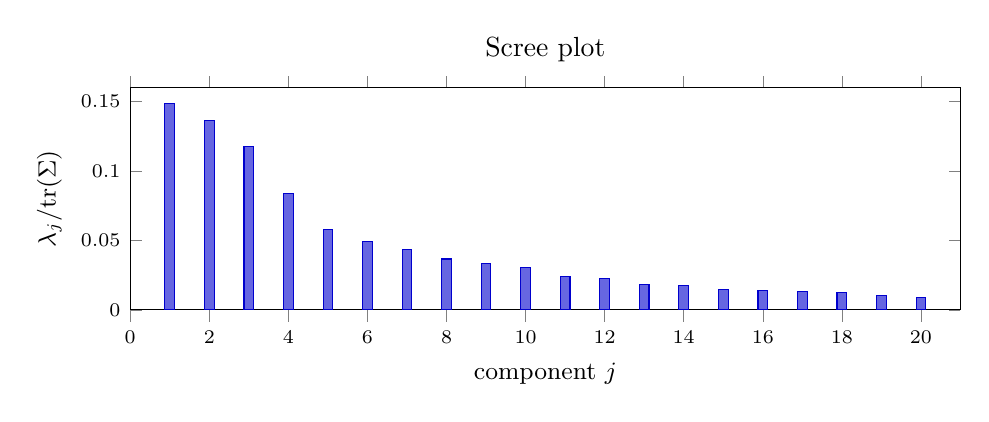
\begin{tikzpicture}
    \begin{axis}[width=\linewidth, height=4.4cm, ybar, bar width=3.5pt, scaled y ticks=false,
        yticklabel style={/pgf/number format/fixed, /pgf/number format/precision=2},
        xmin=0, xmax=21, ymin=0, ymax=0.16, title={Scree plot},
        xlabel={component $j$}, ylabel={$\lambda_j / \mathrm{tr}(\Sigma)$},
        tick label style={font=\scriptsize}, label style={font=\small}]
    \addplot[fill=MediumBlue!60, draw=MediumBlue] coordinates {(1,0.1489) (2,0.1362) (3,0.1179) (4,0.0841) (5,0.0578) (6,0.0492) (7,0.0432) (8,0.0366) (9,0.0335) (10,0.0308) (11,0.0237) (12,0.0227) (13,0.0182) (14,0.0177) (15,0.0147) (16,0.0141) (17,0.0132) (18,0.0125) (19,0.0102) (20,0.0091)};
    \end{axis}
    \end{tikzpicture}
    \column{0.5\linewidth}
    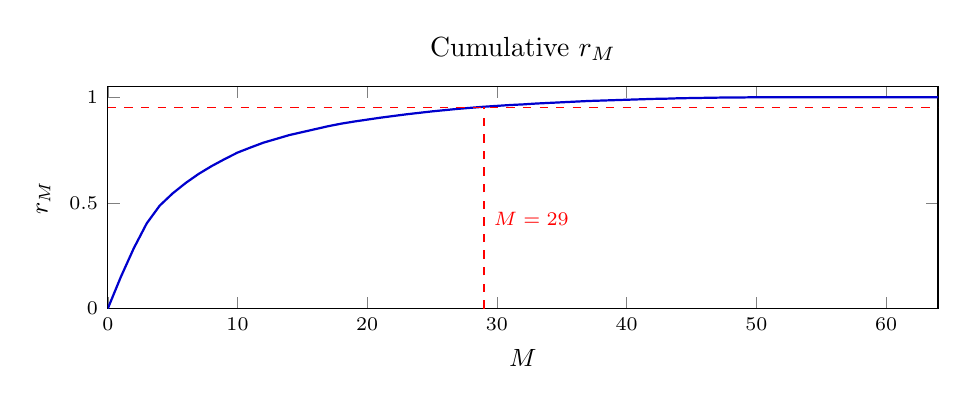
\begin{tikzpicture}
    \begin{axis}[width=\linewidth, height=4.4cm, xmin=0, xmax=64, ymin=0, ymax=1.05,
        title={Cumulative $r_M$}, xlabel={$M$}, ylabel={$r_M$},
        tick label style={font=\scriptsize}, label style={font=\small}]
    \addplot[thick, MediumBlue, mark=none] coordinates {(0,0) (1,0.149) (2,0.285) (3,0.403) (4,0.487) (5,0.545) (6,0.594) (7,0.637) (8,0.674) (9,0.707) (10,0.738) (11,0.762) (12,0.785) (13,0.803) (14,0.821) (15,0.835) (16,0.849) (17,0.863) (18,0.875) (19,0.885) (20,0.894) (21,0.903) (22,0.911) (23,0.919) (24,0.926) (25,0.933) (26,0.939) (27,0.945) (28,0.950) (29,0.955) (30,0.959) (31,0.963) (32,0.966) (33,0.970) (34,0.973) (35,0.976) (36,0.979) (37,0.982) (38,0.984) (39,0.986) (40,0.988) (41,0.990) (42,0.992) (43,0.993) (44,0.995) (45,0.996) (46,0.997) (47,0.998) (48,0.999) (49,0.999) (50,1.000) (64,1.000)};
    \draw[dashed, Red] (axis cs:0,0.95) -- (axis cs:64,0.95);
    \draw[dashed, Red] (axis cs:29,0) -- (axis cs:29,0.955);
    \node[font=\scriptsize, anchor=north west, Red] at (axis cs:29,0.5) {$M = 29$};
    \end{axis}
    \end{tikzpicture}
    \end{columns}
    \small
    Handwritten digits, \texttt{sklearn.datasets.load\_digits}: $N = 1797$ images of $8\times 8$ pixels, so $D = 64$. The pixels are centered and left unscaled.
    \begin{multiequation}
        r_M = \cfrac{\sum_{j=1}^M \lambda_j}{\sum_{j=1}^D \lambda_j}, \qquad r_{13} = 0.803, \quad r_{21} = 0.903, \quad r_{29} = 0.955, \quad r_{41} = 0.990
    \end{multiequation}
    The scree plot shows no sharp elbow for these data. A variance threshold gives a definite $M$.
\end{frame}


% https://www2.imm.dtu.dk/pubdb/edoc/imm4000.pdf
\begin{frame}{Using Singular Value Decomposition for PCA}
    
        After centering the dataset, the covariance matrix is $\Sigma = \cfrac{1}{N}\Xbf\Xbf^\top$ in matrix representation.

    Let $\Ubf$ be the matrix of eigenvectors, sorted by eigenvalue with the largest first. The PCA transformation of the data is $\Zbf = \Ubf^\top \Xbf$. Keeping the first $M$ rows of $\Zbf$ projects the data onto $M$ dimensions.
    
    \begin{tblock}{}
        When using the data matrix $\Xbf$ notation, we follow a convention where the rows denote the features from 1 to D and the columns are the samples from 1 to N. 
    \end{tblock}

\end{frame}



\begin{frame}{Using Singular Value Decomposition for PCA}
    \large
    With $\Xbf \in \Rbb^{D\times N}$ centered, take $\Xbf = \Qbf\boldsymbol{\Gamma}\Vbf^\top$ with $\Qbf \in \Rbb^{D\times D}$, $\boldsymbol{\Gamma} \in \Rbb^{D\times N}$, $\Vbf \in \Rbb^{N\times N}$.
    \begin{multiequation}
        \Sigma &= \cfrac{1}{N}\Xbf\Xbf^\top = \Qbf\left(\cfrac{1}{N}\boldsymbol{\Gamma}\boldsymbol{\Gamma}^\top\right)\Qbf^\top \;\Rightarrow\; \Ubf = \Qbf, \quad \lambda_j = \cfrac{\gamma_j^2}{N}\\
        \Zbf &= \Ubf^\top\Xbf = \Qbf^\top\Qbf\,\boldsymbol{\Gamma}\Vbf^\top = \boldsymbol{\Gamma}\Vbf^\top
    \end{multiequation}
    Row $j$ of $\Zbf$ is $\gamma_j \mathbf{v}_j^\top$. Keep the first $M$ rows.
    \begin{tblock}{Why SVD in practice}
        SVD never forms $\Xbf\Xbf^\top$, whose condition number is the square of the condition number of $\Xbf$. The small eigenvalues keep more of their correct digits.
    \end{tblock}
\end{frame}


\begin{frame}{PCA as an Algorithm}
    \large
    \textbf{Fit} on the training data $\Xbf_{\text{train}} \in \Rbb^{D\times N}$:
    \begin{enumerate}
                \item Compute $\boldsymbol{\mu}$. Set $\mathbf{S} = \mathrm{diag}(\sigma_1, \ldots, \sigma_D)$ when the features carry different units, and $\mathbf{S} = \mathbf{I}$ otherwise.
        \item Standardize: $\Xbf \leftarrow \mathbf{S}^{-1}(\Xbf - \boldsymbol{\mu}\mathbf{1}^\top)$.
        \item SVD $\Xbf = \Qbf\boldsymbol{\Gamma}\Vbf^\top$, so $\lambda_j = \gamma_j^2/N$.
        \item Choose $M$ from $r_M$. $\Bbf$ holds the first $M$ columns of $\Qbf$.
    \end{enumerate}
    \textbf{Transform} a new point $\xbf$:
    \begin{multiequation}
        \zbf = \Bbf^\top\mathbf{S}^{-1}(\xbf - \boldsymbol{\mu}), \qquad \hat{\xbf} = \boldsymbol{\mu} + \mathbf{S}\Bbf\zbf
    \end{multiequation}
    \begin{tblock}{}
        $\boldsymbol{\mu}$, $\mathbf{S}$ and $\Bbf$ come from the training set. Refitting them on test data leaks information into the evaluation.
    \end{tblock}
\end{frame}

\begin{sectionframe}{\faCalculator}{PCA by Hand}
\end{sectionframe}

\begin{frame}{PCA by Hand: Data and Centering}
    \large
    Four samples with two features in the same units. We center and skip the rescaling.
    \begin{center}
    \renewcommand{\arraystretch}{1.3}
    \begin{tabular}{c|cc|cc}
        $i$ & $x_{i1}$ & $x_{i2}$ & $x_{i1} - \mu_1$ & $x_{i2} - \mu_2$ \\ \hline
        1 & $-13$ & $-2$ & $-15$ & $-5$  \\
        2 & $1$   & $-4$ & $-1$  & $-7$  \\
        3 & $9$   & $2$  & $7$   & $-1$  \\
        4 & $11$  & $16$ & $9$   & $13$  \\ \hline
        mean & $2$ & $3$ & $0$  & $0$
    \end{tabular}
    \end{center}
    \begin{multiequation}
        \boldsymbol{\mu} = \cfrac{1}{4}\begin{bmatrix} -13 + 1 + 9 + 11 \\ -2 - 4 + 2 + 16\end{bmatrix} = \begin{bmatrix} 2 \\ 3 \end{bmatrix}
    \end{multiequation}
\end{frame}

\begin{frame}{PCA by Hand: Covariance Matrix}
    \large
    \begin{multiequation}
        \Sigma_{11} &= \tfrac{1}{4}\left[(-15)^2 + (-1)^2 + 7^2 + 9^2\right] = \tfrac{356}{4} = 89\\
        \Sigma_{12} &= \tfrac{1}{4}\left[(-15)(-5) + (-1)(-7) + (7)(-1) + (9)(13)\right] = \tfrac{192}{4} = 48\\
        \Sigma_{22} &= \tfrac{1}{4}\left[(-5)^2 + (-7)^2 + (-1)^2 + 13^2\right] = \tfrac{244}{4} = 61
    \end{multiequation}
    \begin{multiequation}
        \Sigma = \begin{bmatrix} 89 & 48 \\ 48 & 61 \end{bmatrix}, \qquad \mathrm{tr}(\Sigma) = 150, \qquad \det(\Sigma) = 3125
    \end{multiequation}
    The positive off-diagonal entry says the two features rise together. Their correlation is $48/\sqrt{89\cdot 61} = 0.65$.
\end{frame}


\begin{frame}{PCA by Hand: Eigenvalues and Eigenvectors}
    \large
    \begin{multiequation}
        \det(\Sigma - \lambda\mathbf{I}) &= (89-\lambda)(61-\lambda) - 48^2 = \lambda^2 - 150\lambda + 3125 = 0\\
        &\Rightarrow\; (\lambda - 125)(\lambda - 25) = 0 \;\Rightarrow\; \lambda_1 = 125,\ \ \lambda_2 = 25
    \end{multiequation}
    \begin{columns}
    \column{0.5\linewidth}
    $\lambda_1 = 125$:
    \begin{multiequation}
        \begin{bmatrix} -36 & 48 \\ 48 & -64 \end{bmatrix}\bbf_1 = \mathbf{0} \;\Rightarrow\; \bbf_1 = \begin{bmatrix} 0.8 \\ 0.6 \end{bmatrix}
    \end{multiequation}
    \column{0.5\linewidth}
    $\lambda_2 = 25$:
    \begin{multiequation}
        \begin{bmatrix} 64 & 48 \\ 48 & 36 \end{bmatrix}\bbf_2 = \mathbf{0} \;\Rightarrow\; \bbf_2 = \begin{bmatrix} -0.6 \\ 0.8 \end{bmatrix}
    \end{multiequation}
    \end{columns}
    \medskip
    Checks: $\lambda_1 + \lambda_2 = 150 = \mathrm{tr}(\Sigma)$, $\lambda_1\lambda_2 = 3125 = \det(\Sigma)$, $\bbf_1^\top\bbf_2 = -0.48 + 0.48 = 0$.

    PC1 explains $125/150 = 83.3\%$ of the variance.
\end{frame}



\begin{frame}{PCA by Hand: Project onto PC1 and Reconstruct}
    \large
    $z_i = \bbf_1^\top(\xbf_i - \boldsymbol{\mu}), \qquad \hat{\xbf}_i = \boldsymbol{\mu} + z_i\,\bbf_1$
    \begin{center}
    \renewcommand{\arraystretch}{1.3}
    \begin{tabular}{c|c|c|c|c}
        $i$ & $z_i$ & $\hat{\xbf}_i$ & $\xbf_i - \hat{\xbf}_i$ & $\|\xbf_i - \hat{\xbf}_i\|^2$ \\ \hline
        1 & $-12 - 3 = -15$     & $(-10, -6)$ & $(-3, 4)$ & 25 \\
        2 & $-0.8 - 4.2 = -5$   & $(-2, 0)$   & $(3, -4)$ & 25 \\
        3 & $5.6 - 0.6 = 5$     & $(6, 6)$    & $(3, -4)$ & 25 \\
        4 & $7.2 + 7.8 = 15$    & $(14, 12)$  & $(-3, 4)$ & 25
    \end{tabular}
    \end{center}
    \begin{multiequation}
        \tfrac{1}{4}\textstyle\sum_i z_i^2 = \tfrac{500}{4} = 125 = \lambda_1, \qquad \text{Error} = \tfrac{100}{4} = 25 = \lambda_2
    \end{multiequation}
    The residuals point along $\pm\bbf_2$. The 1-D code discards the variance along PC2 and nothing more.
\end{frame}


\begin{frame}{PCA by Hand: The Picture}
    \begin{center}
    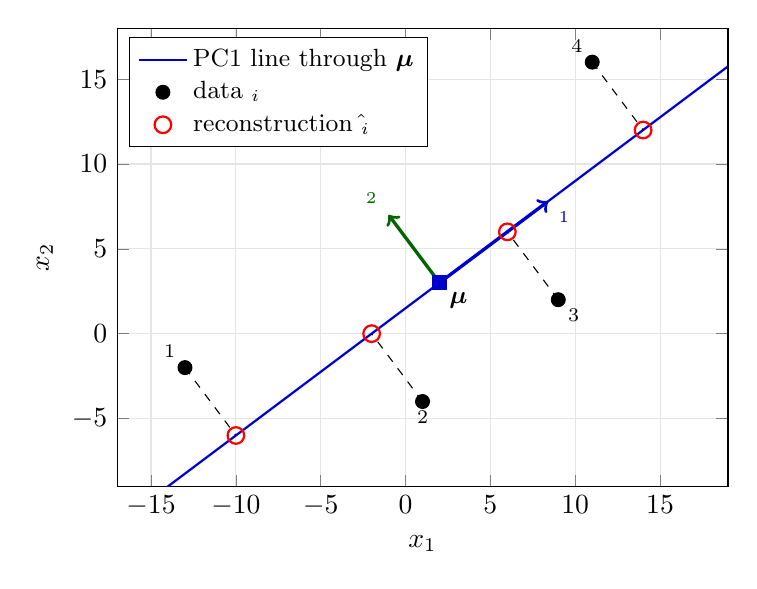
\begin{tikzpicture}
    \begin{axis}[width=11cm, height=7.4cm, axis equal image,
        xmin=-17, xmax=19, ymin=-9, ymax=18, grid=both, grid style={gray!20},
        xlabel={$x_1$}, ylabel={$x_2$},
        legend style={font=\small, at={(0.02,0.98)}, anchor=north west}, legend cell align=left]
        \addplot[thick, MediumBlue, domain=-17:19, samples=2] {3 + 0.75*(x - 2)};
        \addlegendentry{PC1 line through $\boldsymbol{\mu}$}
        \addplot[only marks, mark=*, mark size=2.5pt, black] coordinates {(-13,-2) (1,-4) (9,2) (11,16)};
        \addlegendentry{data $\xbf_i$}
        \addplot[only marks, mark=o, mark size=3pt, thick, Red] coordinates {(-10,-6) (-2,0) (6,6) (14,12)};
        \addlegendentry{reconstruction $\hat{\xbf}_i$}
        \draw[dashed] (axis cs:-13,-2) -- (axis cs:-10,-6);
        \draw[dashed] (axis cs:1,-4) -- (axis cs:-2,0);
        \draw[dashed] (axis cs:9,2) -- (axis cs:6,6);
        \draw[dashed] (axis cs:11,16) -- (axis cs:14,12);
        \draw[->, very thick, MediumBlue] (axis cs:2,3) -- (axis cs:8.4,7.8) node[pos=1, anchor=north west, font=\small] {$\bbf_1$};
        \draw[->, very thick, DarkGreen] (axis cs:2,3) -- (axis cs:-1,7) node[pos=1, anchor=south east, font=\small] {$\bbf_2$};
        \addplot[only marks, mark=square*, mark size=2.5pt, MediumBlue] coordinates {(2,3)};
        \node[font=\small, anchor=north west] at (axis cs:2,3) {$\boldsymbol{\mu}$};
        \node[font=\scriptsize, anchor=south east] at (axis cs:-13,-2) {1};
        \node[font=\scriptsize, anchor=north] at (axis cs:1,-4) {2};
        \node[font=\scriptsize, anchor=north west] at (axis cs:9,2) {3};
        \node[font=\scriptsize, anchor=south east] at (axis cs:11,16) {4};
    \end{axis}
    \end{tikzpicture}
    \end{center}
\end{frame}

\begin{frame}[fragile]{PCA by Hand: Checking with Python}
\begin{minted}[fontsize=\footnotesize, bgcolor=LightGray]{python}
import numpy as np
from sklearn.decomposition import PCA

X = np.array([[-13, -2], [1, -4], [9, 2], [11, 16]])  # N x D
Xc = X - X.mean(axis=0)
Sigma = Xc.T @ Xc / len(X)            # 1/N, as on the slides
lam, B = np.linalg.eigh(Sigma)        # ascending order
print(lam)                            # [ 25. 125.]

pca = PCA().fit(X)
print(pca.explained_variance_)        # [166.67  33.33], uses 1/(N-1)
print(pca.explained_variance_ratio_)  # [0.833 0.167], same ratio
print(pca.components_)                # rows are b1, b2, sign may flip
print(pca.transform(X)[:, 0])         # z_i = [-15. -5.  5. 15.]
\end{minted}
\small
\textbf{Conventions to watch.} \texttt{sklearn} stores samples as rows, the transpose of our $\Xbf$, and divides by $N-1$. An eigenvector is fixed up to sign, so $-\bbf_1$ is an equally valid answer.
\end{frame}

\begin{sectionframe}{\faExclamationTriangle}{Limitations and Beyond PCA}
\end{sectionframe}

\begin{frame}{To Standardize or Not}
    \large
    Rescale $x_1$ of the worked example by 10, say centimeters to millimeters:
    \begin{multiequation}
        \Sigma' = \begin{bmatrix} 8900 & 480 \\ 480 & 61 \end{bmatrix} \;\Rightarrow\; \lambda_1' = 8926.0, \quad r_1 = 0.996
    \end{multiequation}
    PC1 now lies $3.1^\circ$ off the $x_1$ axis and explains 99.6\% of the variance, up from 83.3\%. The points are the same. A change of unit moved PC1.
    \begin{tblock}{Rule of thumb}
        Standardize when the features carry different units, such as meters and kilograms. Keep the raw scale when the units match and the spread itself carries meaning, as with pixel intensities.
    \end{tblock}
    \small
    A pixel that stays blank across the data set has $\sigma_j = 0$, and $x_{ij}/\sigma_j$ is undefined. The digits data contain three such pixels. \texttt{StandardScaler} leaves those columns unscaled.
\end{frame}


\begin{frame}{PCA Ignores the Labels}
    \begin{columns}
    \column{0.5\linewidth}
    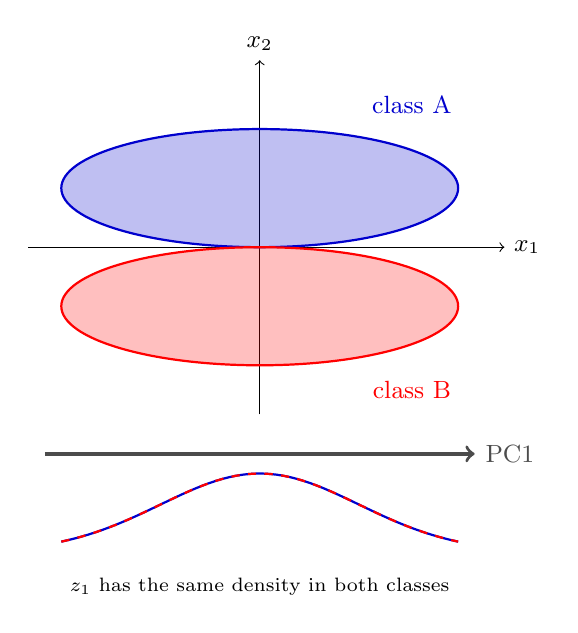
\begin{tikzpicture}[xscale=0.42, yscale=1.25]
        \draw[->] (-7,0) -- (7.4,0) node[right, font=\small] {$x_1$};
        \draw[->] (0,-1.7) -- (0,1.9) node[above, font=\small] {$x_2$};
        \fill[MediumBlue, opacity=0.25] (0,0.6) ellipse (6 and 0.6);
        \draw[MediumBlue, thick] (0,0.6) ellipse (6 and 0.6);
        \fill[Red, opacity=0.25] (0,-0.6) ellipse (6 and 0.6);
        \draw[Red, thick] (0,-0.6) ellipse (6 and 0.6);
        \node[MediumBlue, font=\small] at (4.6,1.45) {class A};
        \node[Red, font=\small] at (4.6,-1.45) {class B};
        \draw[->, very thick, black!70] (-6.5,-2.1) -- (6.5,-2.1) node[right, font=\small] {PC1};
        \draw[MediumBlue, thick, domain=-6:6, samples=60] plot (\x, {-3.1 + 0.8*exp(-\x*\x/18)});
        \draw[Red, thick, dashed, domain=-6:6, samples=60] plot (\x, {-3.1 + 0.8*exp(-\x*\x/18)});
        \node[font=\scriptsize, align=center] at (0,-3.45) {$z_1$ has the same density in both classes};
    \end{tikzpicture}
    \column{0.5\linewidth}
    Two classes with equal priors. Within a class, $\sigma = 3$ along $x_1$ and $\sigma = 0.3$ along $x_2$. The class means sit at $x_2 = \pm 0.6$.
    \begin{multiequation}
        \mathrm{Var}(x_1) &= 3^2 = 9\\
        \mathrm{Var}(x_2) &= \underbrace{0.3^2}_{\text{within}} + \underbrace{0.6^2}_{\text{between}} = 0.45
    \end{multiequation}
    PC1 is the $x_1$ axis and keeps $9/9.45 = 95\%$ of the variance. A classifier that sees $z_1$ alone is right half the time.
    \begin{tblock}{}
        PCA ranks directions by spread. Here the class information sits in the low-variance direction. LDA uses the labels and picks $x_2$.
    \end{tblock}
    \end{columns}
\end{frame}


\begin{frame}{Beyond PCA}
    \footnotesize
    \renewcommand{\arraystretch}{1.3}
    \begin{center}
    \begin{tabular}{l|l|>{\raggedright\arraybackslash}p{5.2cm}|>{\raggedright\arraybackslash}p{4.4cm}}
        Method & Map & What it preserves & Embeds a new point? \\ \hline
        PCA & linear & directions of largest variance & yes, $\Bbf^\top(\xbf - \boldsymbol{\mu})$ \\
        Kernel PCA & nonlinear & variance in a kernel feature space & yes, via kernel values with the training points \\
        ICA & linear & independent, non-Gaussian sources & yes, the unmixing matrix \\
        t-SNE & nonlinear & local neighborhoods, for 2-D or 3-D plots & no direct map \\
        UMAP & nonlinear & local neighborhoods and part of the global layout & yes, approximate \\
        Autoencoder & nonlinear & reconstruction through a bottleneck & yes, the encoder \\
    \end{tabular}
    \end{center}
    \begin{tblock}{A link back to PCA}
        A linear autoencoder trained with squared error spans the subspace of the top $M$ principal components (Baldi and Hornik, 1989). Nonlinear activations let it learn a curved manifold.
    \end{tblock}
    Cluster sizes and gaps in a t-SNE plot carry little meaning. Read the neighborhoods.
\end{frame}


      %------------------------------------------------
    
    \begin{frame}[containsverbatim]{Python Notebook}
    \begin{center}
    \small
    { \color{Red}{\url{https://github.com/rahulbhadani/CPE486586_FA25/blob/main/Code/CPE486586_Ch10_Dimensionality_Reduction.ipynb}}}
    \end{center}
    \end{frame}
    
    %------------------------------------------------
    
    \begin{frame}
        \Huge{\centerline{\color{MediumBlue}\textbf{The End}}}
    \end{frame}

\end{document}